\documentclass[a4paper]{article}

%Inicio, onde declara quais pacotes serão utilizados no projeto
\usepackage[brazilian]{babel} %Para sair ja escrito, tabela e não table
\usepackage[utf8]{inputenc} % Para usar acentos
\usepackage{mathptmx} % math functions!
\usepackage{amsmath} % moar math
\usepackage[11pt]{moresize} % different letters sizes
\usepackage{float} % enables accurate location of tables
\usepackage{caption} % to make personalized captions
\usepackage{graphicx} % required for the inclusion of images
\usepackage[margin=0.8in]{geometry} %Faz uma correção das margens


\title{Experimento 02 \\ Pêndulo de Torção}
\author{F 229 \\ \textsc{Grupo 1}}
\date{17 de Setembro, 2014}


\begin{document} % actually starts the document here
\maketitle

% members of the group
\begin{center}
	\begin{tabular}{l r l}
		Integrantes: & Henrique Noronha Facioli & 157986 \\
		& Guilherme Lucas da Silva & 155618 \\
		& Beatriz Sechin Zazulla & 154779 \\
		& Lucas Alves Racoci & 156331 \\
		& Isadora Sophia Garcia Rodopoulos & 158018 \\
	\end{tabular}
\end{center}




\section{Resumo}

Neste experimento, estudamos um pêndulo de torção, cujo período $T$ é determinado pela equação:

\begin{align}
   T = \sqrt{\frac{8 \pi I_0}{4 G r}}\
   \label{eq:Periodo}
\end{align}

Neste estudo, medimos variações de $T$ em função do comprimento do fio $L$ ,que tem liberdade de torção, com o auxilio de um photogate ligado a um cronômetro inteligente, formulando assim um gráfico linearizado da equação acima, tomando os eixos $L$ em função de $T^2$. Além disso, calculamos o momento de inércia $I_0$ do conjunto de três cilindros, supondo que os três tinham a mesma densidade e usando as formulas de volume de cilindro e a massa que nos foi dada.
A partir disso, calculamos o módulo de cisalhamento $G$ do fio de Aço ASTM, porém não obtivemos o valor esperado dentro da faixa de erro, apesar de chegarmos bem perto.


\section{Objetivo}

Este experimento tem como objetivo estudar o comportamento de um pêndulo de torção e determinar o módulo de cisalhamento (com seu respectivo erro) do fio que o compõe. Um pêndulo de torção é uma estrutura que oscila em torno de um eixo que coincide com o fio que o suspende. Obtêm-se facilmente dados sobre o fio em questão, uma vez que grandezas relacionadas a ele, tais como seu módulo de cisalhamento $G$, ou módulo de torção, e raio $r$ estão diretamente ligadas ao período de oscilação do pêndulo como mostra a seguinte equação:


Deste modo, a partir do cálculo do momento de inércia $I_0$, da medição do raio $r$ e de diversos valores para o período $T$, tomando experimentalmente variados comprimentos $L$ para o fio, obtêm-se o módulo de cisalhamento $G$ do mesmo, tal como objetivado.

\section{Procedimentos e coleta de dados}
\subsection{Materiais utilizados}
Foram utilizados os seguintes materiais para a execução do experimento:

\begin{enumerate} 
	\item Pêndulo de torção (fio de suspensão e peso metálico circular preso na ponta do fio);
	\item Micrômetro;
	\item Paquímetro;
	\item Trena de precisão milimétrica;
	\item Photogate;
	\item Cronômetro inteligente;
 \end {enumerate} 
 
 \subsection{Procedimento}
De posse dos materiais, iniciamos o experimento aferindo as dimensões (raios e alturas) da estrutura pendular circular, utilizando o paquímetro, para que conseguíssemos determinar seu momento de inércia. A massa de tal estrutura nos foi dada já mensurada em laboratório. Em seguida, medimos o diâmetro do fio que suspendia o pêndulo com o micrômetro, a fim de determinar seu raio $r$.

\begin{figure}[!htbp]
	\centering
	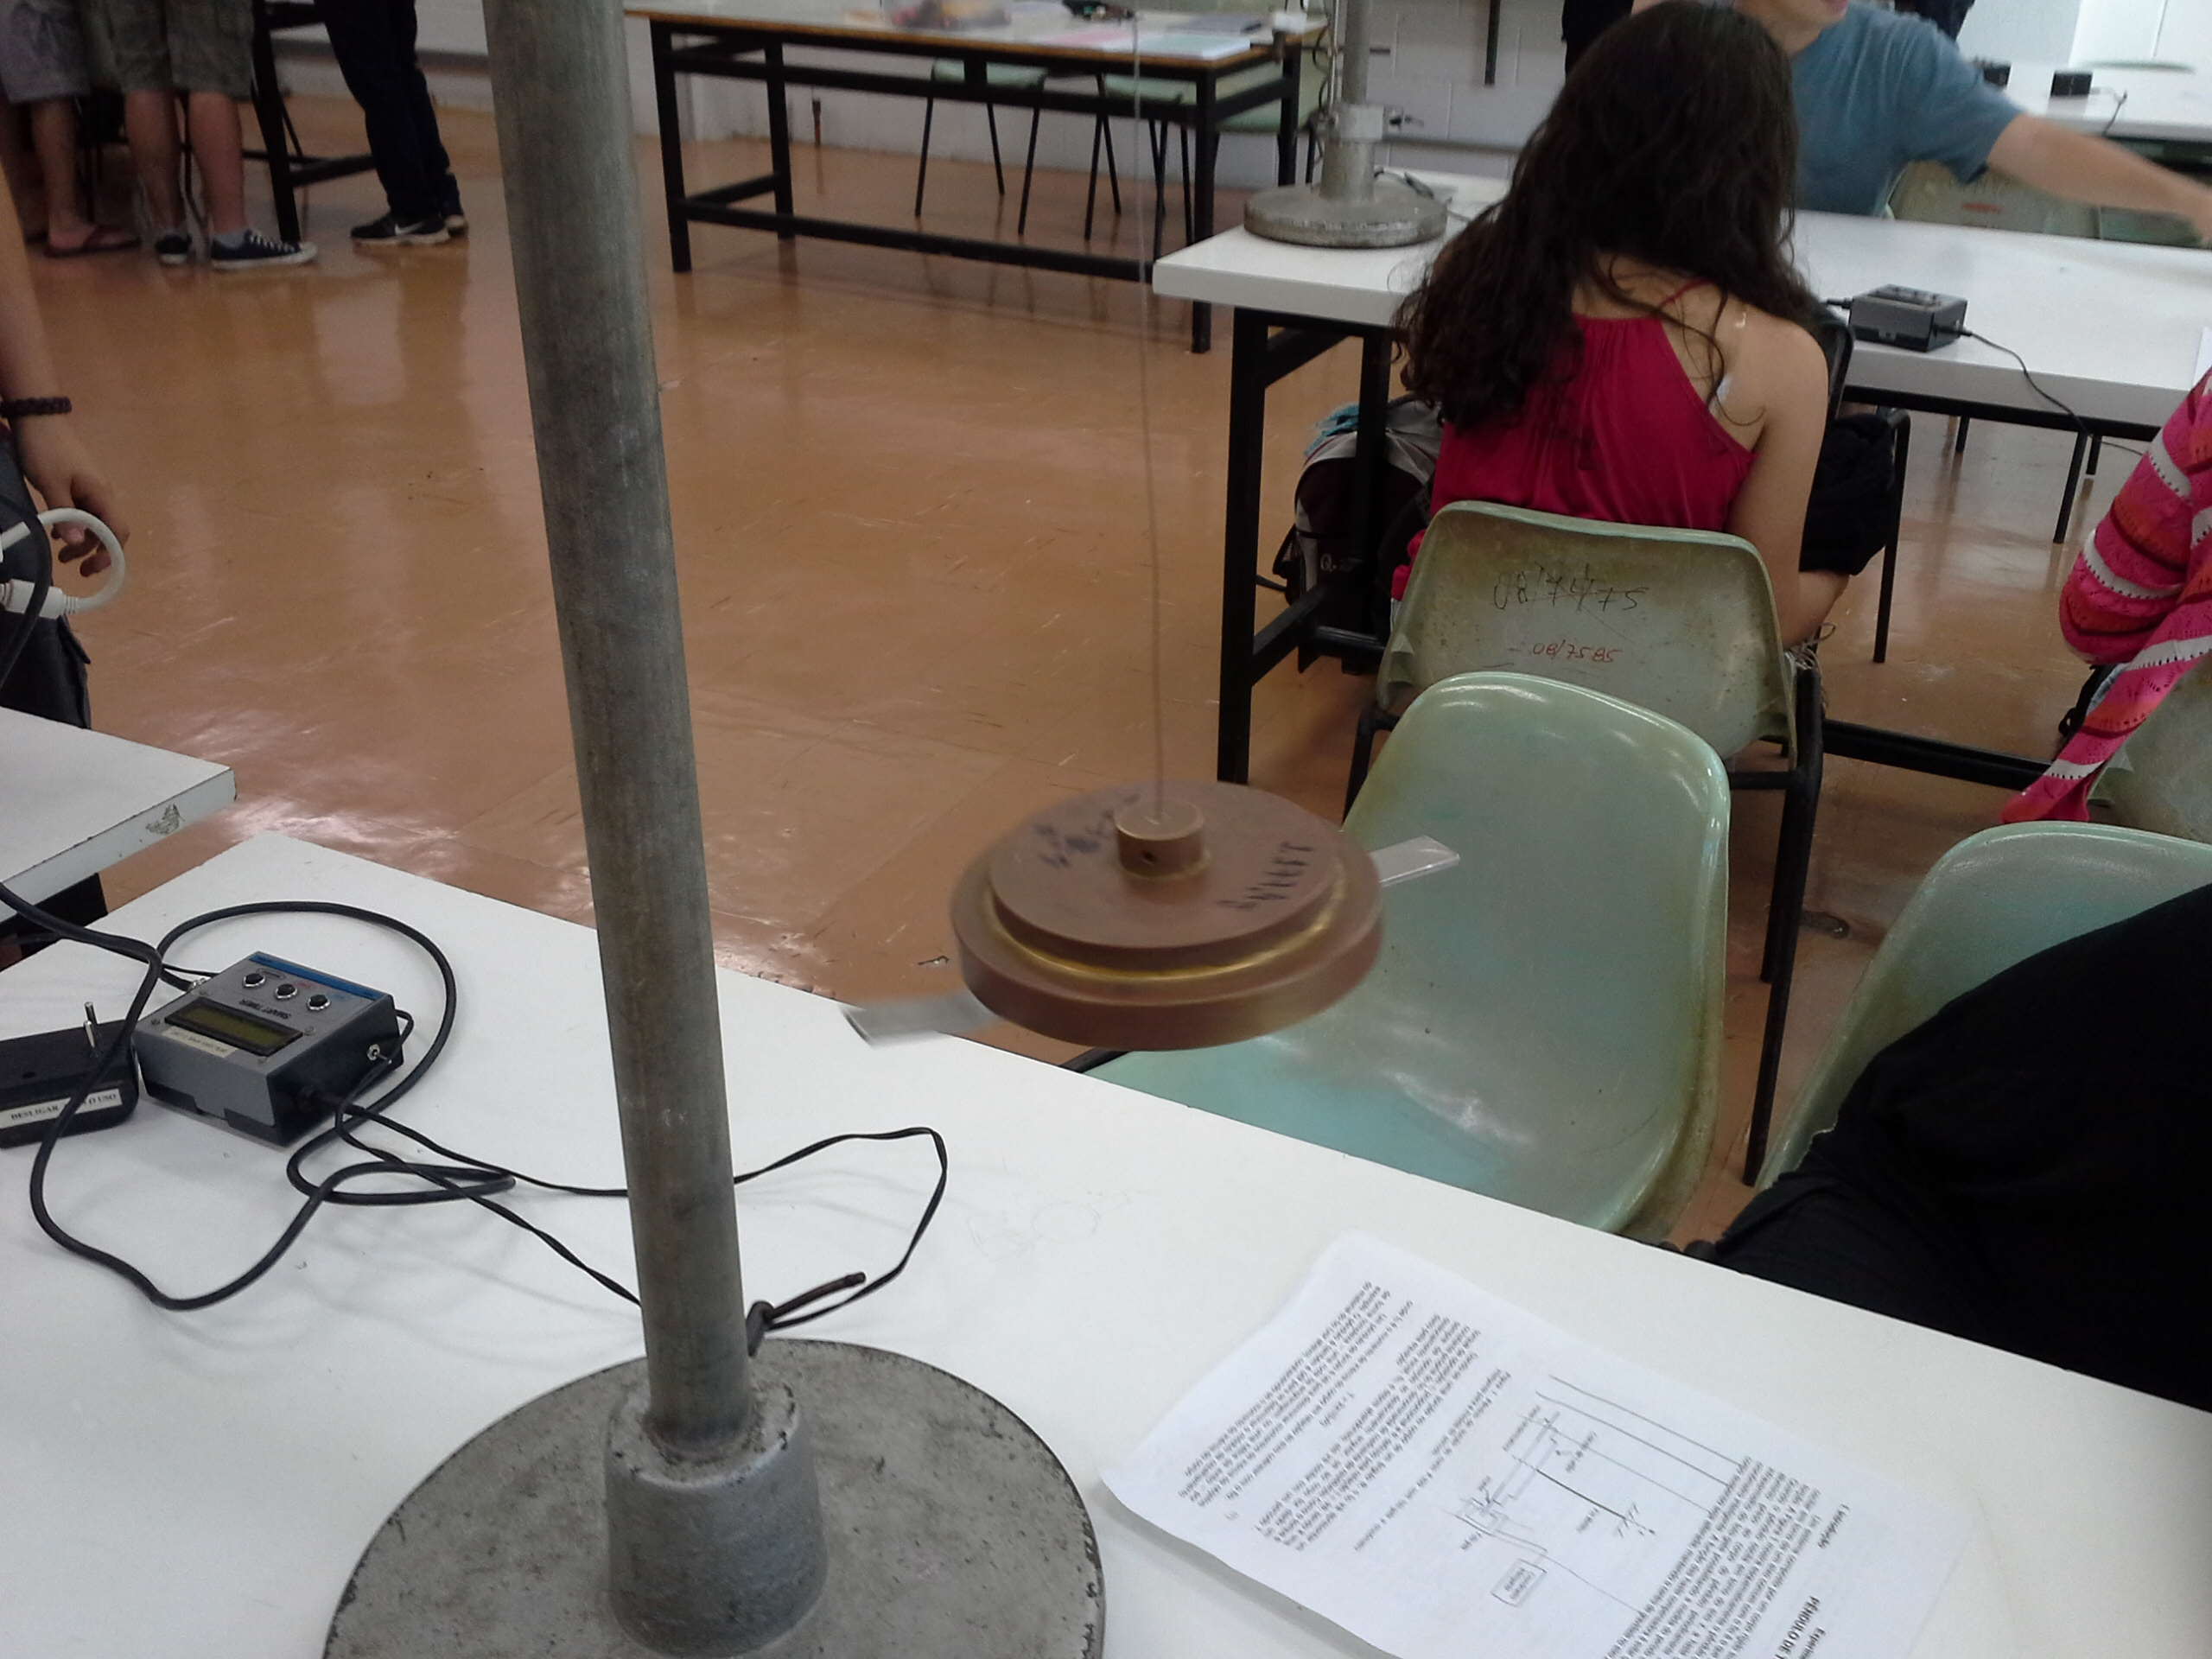
\includegraphics[scale=0.1]{1.jpg}
	\caption{Montagem do experimento}
	\label{fig:cilindro}
\end{figure}

Conectamos o photogate ao cronômetro inteligente e iniciamos as medidas. Para cada, utilizávamos a trena de precisão milimétrica para determinar o comprimento $L$ do fio que suspendia o pêndulo. Oscilávamos o pêndulo de torção por vinte vezes passando pelo photogate ligado ao cronômetro inteligente, que no modo “Pêndulo” nos dava o período de cada oscilação, usado nas equações deste movimento em função do comprimento $L$ determinado. Esse processo se repetiu por cerca de seis medições, número que se mostrou satisfatório para a obtenção dos dados.

\begin{table}[!htbp]
\centering
	    \caption{Valores de medidas do periodo $T$ para cada comprimento $L$ do fio}
	    \begin{tabular}{|c|l|l|l|l|l|l|l|l|l|l|l|l|}
	    \hline
	     ~	 &	 $L_1$    & $\Delta_{L_1}$  & $L_2$     & $\Delta_{L_2}$  & $L_3$     & $\Delta_{L_3}$  & $L_4$     & $\Delta_{L_4}$  & $L_5$     & $\Delta_{L_5}$  & $L_6$     & $\Delta_{L_6}$  \\ \\cline{2-13}
	    ~	&	0,358  & 0,001  & 0,203  & 0,001  & 0,258  & 0,001  & 0,464  & 0,001  & 0,398  & 0,001  & 0,589  & 0,001  \\ \hline
	    N	&	$T_{1n}$      & $\Delta_T$   & $T_{2n}$      & $\Delta_T$   & $T_{3n}$      & $\Delta_T$   & $T_{4n}$      & $\Delta_T$   & $T_{5n}$      & $\Delta_T$   & $T_{6n}$      & $\Delta_T$   \\ \hline
		1	&	4,7766 & 0,0001 & 3,6408 & 0,0001 & 4,0712 & 0,0001 & 5,4234 & 0,0001 & 5,0419 & 0,0001 & 6,0831 & 0,0001 \\ \hline
		2	&	4,7731 & 0,0001 & 3,6423 & 0,0001 & 4,0704 & 0,0001 & 5,4212 & 0,0001 & 5,0403 & 0,0001 & 6,0804 & 0,0001 \\ \hline
		3	&	4,774  & 0,0001 & 3,6422 & 0,0001 & 4,0732 & 0,0001 & 5,4228 & 0,0001 & 5,0417 & 0,0001 & 6,0824 & 0,0001 \\ \hline
 		4	&	4,7746 & 0,0001 & 3,6432 & 0,0001 & 4,074  & 0,0001 & 5,4228 & 0,0001 & 5,0429 & 0,0001 & 6,0797 & 0,0001 \\ \hline
  		5	&	4,7737 & 0,0001 & 3,6395 & 0,0001 & 4,0726 & 0,0001 & 5,4229 & 0,0001 & 5,0417 & 0,0001 & 6,0856 & 0,0001 \\ \hline
 		6	&	4,7748 & 0,0001 & 3,6397 & 0,0001 & 4,0726 & 0,0001 & 5,4209 & 0,0001 & 5,0439 & 0,0001 & 6,0816 & 0,0001 \\ \hline
   		7	&	4,7754 & 0,0001 & 3,6396 & 0,0001 & 4,0734 & 0,0001 & 5,4214 & 0,0001 & 5,0426 & 0,0001 & 6,0806 & 0,0001 \\ \hline
    	8	&	4,7747 & 0,0001 & 3,6415 & 0,0001 & 4,0735 & 0,0001 & 5,4221 & 0,0001 & 5,0423 & 0,0001 & 6,0822 & 0,0001 \\ \hline
    	9	&	4,7755 & 0,0001 & 3,6412 & 0,0001 & 4,0729 & 0,0001 & 5,4225 & 0,0001 & 5,0423 & 0,0001 & 6,0814 & 0,0001 \\ \hline
    	10	&	4,7755 & 0,0001 & 3,6407 & 0,0001 & 4,0735 & 0,0001 & 5,4215 & 0,0001 & 5,0425 & 0,0001 & 6,0796 & 0,0001 \\ \hline
    	11	&	4,7763 & 0,0001 & 3,6389 & 0,0001 & 4,0724 & 0,0001 & 5,4223 & 0,0001 & 5,0435 & 0,0001 & 6,0829 & 0,0001 \\ \hline
    	12	&	4,7772 & 0,0001 & 3,6392 & 0,0001 & 4,0726 & 0,0001 & 5,4218 & 0,0001 & 5,0426 & 0,0001 & 6,081  & 0,0001 \\ \hline
    	13	&	4,7765 & 0,0001 & 3,6402 & 0,0001 & 4,0675 & 0,0001 & 5,4207 & 0,0001 & 5,0434 & 0,0001 & 6,0802 & 0,0001 \\ \hline
    	14	&	4,7776 & 0,0001 & 3,6402 & 0,0001 & 4,0692 & 0,0001 & 5,4212 & 0,0001 & 5,0433 & 0,0001 & 6,079  & 0,0001 \\ \hline
    	15	&	4,7763 & 0,0001 & 3,6404 & 0,0001 & 4,0647 & 0,0001 & 5,4241 & 0,0001 & 5,0445 & 0,0001 & 6,0839 & 0,0001 \\ \hline
    	16	&	4,7764 & 0,0001 & 3,6389 & 0,0001 & 4,0644 & 0,0001 & 5,4241 & 0,0001 & 5,0443 & 0,0001 & 6,0814 & 0,0001 \\ \hline
    	17	&	4,7768 & 0,0001 & 3,6446 & 0,0001 & 4,0631 & 0,0001 & 5,4215 & 0,0001 & 5,0449 & 0,0001 & 6,0816 & 0,0001 \\ \hline
    	18	&	4,7752 & 0,0001 & 3,6412 & 0,0001 & 4,065  & 0,0001 & 5,4215 & 0,0001 & 5,0433 & 0,0001 & 6,0805 & 0,0001 \\ \hline
    	19	&	4,7754 & 0,0001 & 3,6415 & 0,0001 & 4,0677 & 0,0001 & 5,4208 & 0,0001 & 5,0442 & 0,0001 & 6,0802 & 0,0001 \\ \hline
    	20	&	4,7756 & 0,0001 & 3,6421 & 0,0001 & 4,062  & 0,0001 & 5,4234 & 0,0001 & 5,0442 & 0,0001 & 6,0804 & 0,0001 \\ \hline
	    \end{tabular}
	    \label{tab:MedidasTeL}
\end{table}

\begin{table}[!htbp]
\centering
	\caption{Valores de medidas do fio obtidas utilizando um manômetro}
	\begin{tabular}{|l|l|}
	\hline
	Raio do fio ($m$) & 0,000275 \\ \hline
	\textbf{$\Delta_r$}	& 0,000005 \\ \hline
	\end{tabular}
	\label{tab:Fio}
\end{table}

\section{Análise e Resultados}

\subsection{Momento de Inércia}
Para calcular o $I_0$ precisamos calcular o momento de inércia $I_n$ de cada um dos cilindros componentes, e para isso tivemos que supor que os cilindros têm a mesma densidade assim pudemos usar a equação:

\begin{align}
	M_k = d V_k = \frac{V_{total}}{M_{total}} V_k\
	\label{eq:MassaDisco}
\end{align}

Onde:
\begin{itemize}
	\item $M_k$ é a massa do k-ézimo cilindro;
	\item $V_{total}$ é a soma dos volumes de cada disco;
	\item $M_{total}$ é a massa dos tres cilindros juntos, e nos foi fornecido, velendo $1,1774\pm0,0001$;
	\item $d$ é a densidade;
	\item $V_k$ é o volume do k-ézimo disco, dado por $V_k = (2 \pi R_k) * h_k$;
\end{itemize}

O erro para essas equações também foi calculado:

Para o cálculo do erro volumétrico:
\begin{align}
   \sigma_V^2 = (2 \pi R h)^2(\sigma_R)+(\pi R^2)(\sigma_h)^2 \
   \label{eq:ErroVolume}
\end{align}

Para o cálculo do erro do volume total $V_t$ dos 3 discos
\begin{align}
   \sigma_{v_t}^2 = \sigma_{v_1}^2 + \sigma_{v_2}^2 + \sigma_{v_3}^2\
   \label{eq:ErroVolumeTotal}
\end{align}

Para o cálculo do erro do momento de inércia $I_0$
\begin{align}
   \sigma_{I_0}^2 = (\frac{R^2}{2})^2 (\sigma_{v_1})^2 +(M R^2)(\sigma_R)^2\
   \label{eq:MomentoInercia}
\end{align}

Todos os resultados são expressos nas seguintes tabelas:

\begin{table}[!htbp]
\centering
    \caption{Características gerais do cilindro de maior tamanho}
    \begin{tabular}{|l|l|l|l|l|l|}
    \hline
    ~      & Raio ($m$) & Altura ($m$) & Volume ($m^3$) & Massa ($Kg$) & Momento Inércia (Kg*$m^3$) \\ \hline
    Medida & 0,04990	&	0,01230	&	0,0000962	&	0,814	&	0,001013 \\ \hline
    Erro   & 0,00003	&	0,00005	&	0,0000004	&	0,005	&	0,000006 \\ \hline
    \end{tabular}
    \label{tab:CilindroMaior}
\end{table}

\begin{table}[!htbp]
\centering
    \caption{Características gerais do cilindro de tamanho médio}
    \begin{tabular}{|c|l|l|l|l|l|}
    \hline
    ~      & Raio ($m$) & Altura ($m$) & Volume ($m^3$) & Massa ($Kg$) & Momento Inércia (Kg*$m^3$) \\ \hline
    Medida & 0,04000  & 0,007900	&	0,0000397	&	0,336	&	0,000269                \\ \hline
    Erro   & 0,00003	&	0,00007	&	0,0000004	&	0,003	&	0,000003               \\ \hline
    \end{tabular}
    \label{tab:CilindroMeio}
\end{table}

\begin{table}[!htbp]
\centering
    \caption{Características gerais do cilindro de menor tamanho}
    \begin{tabular}{|l|l|l|l|l|l|}
    \hline
    ~      & Raio ($m$) & Altura ($m$) & Volume ($m^3$) & Massa ($Kg$) & Momento Inércia (Kg*$m^3$) \\ \hline
    Medida & 0,01005  & 0,0102     & 0,00000324  & 0,0274     & 0,00000138                \\ \hline
    Erro   & 0,00003  & 0,0001     & 0,00000004  & 0,0003     & 0,00000002                \\ \hline
    \end{tabular}
    \label{tab:CilindroMenor}
\end{table}

A partir desse dados, foi possível calcular o Momento de Inércia $I_0$ total:

$$I_0 \mp \sigma_{I_0} = (1,284\mp0,006)*10^-3 Kg*m^2$$

\subsection{Módulo de Cisalhamento}

Para obter o módulo de cisalhamento $G$ através da equação~\ref{eq:Periodo}, primeiro tivemos que linearizar a equação:

\begin{align}
	T^2 = \frac{8 \pi I_0 L}{G r^4 } \Leftrightarrow T^2 G r^4 = 8 \pi I_0 L \Leftrightarrow \underset{y}{\underbrace{L}} =\underset{a}{\underbrace{\frac{G r^4}{8 \pi I_0}}} *\underset{x}{\underbrace{{T^2}}}\
	\label{eq:Cisalhamento}
\end{align}

Para isso escolhemos $y = L$ e $x = T^2$, assim a relação entre o modulo de cisalhamento e o coeficiente angular a ficam assim:

\begin{align}
	a = \frac{G r^4}{8 \pi I_0} \Leftrightarrow G = \frac{a 8 \pi I_0}{r^4}\
	\label{eq:CoeficienteLinear}
\end{align}

Onde:
\begin{itemize}
	\item $I_0 = \sum_{k=1}^{3}(I_k)$ é o momento de inércia total, soma dos momentos de inércia de todos os cilindros, já que todos estão girando no mesmo eixo;
	\item $R$ é o raio do cilindro;
	\item $a$ é o coeficiente linear do gráfico $L x T^2$;
\end{itemize}

Para obter o coeficiente angular, aplicamos o método dos mínimos quadrados utilizando os dados da Tabela ~\ref{tab:MedidasTeL}, calculando-se o desvio padrão, o erro estatístico, juntando com o erro instrumental e já propagando o erro de $T$ para $T^2$ com a fórmula $\sigma_{T^2_m}^2 = 2 \overline{T_m} \sigma_{\overline{T_m}}$, em que $\overline{T_m}$ é a media dos $n$ $T$'s da Tabela ~\ref{tab:MedidasTeL}. A partir desses dados foi possível montar a Tabela 6 e traçar o gráfico ilustrado na Figura 2.

\begin{table}[!htbp]
\centering
	\caption{Dados para a construção do gráfico}
    \begin{tabular}{|c|c|c|c|c|c|c|}
    \hline
    $M$  & 1            & 2            & 3            & 4            & 5            & 6            \\ \hline
    $L (x 10^{-1}m)$  & $(3,58 \pm 0,01)$ & $(2,03 \pm 0,01) $ & $(2,58 \pm 0,01) $ & $(4,64 \pm 0,01) $ & $(3,98 \pm 0,01) $ & $(5,89 \pm 0,01) $ \\ \hline
    $T^2 (x 10s^2)$ & $(2,28 \pm 0,03)$ & $(1,326 \pm 0,004) $ & $(1,66 \pm 0,03)x10$  & $(2,94\pm0,01) $ & $(2,54 \pm 0,09) $   & $(3,70\pm0,01) x10$  \\ \hline
    \end{tabular}
    \label{tab:grafico}
\end{table}

Usado Método dos mínimos quadrados, obtêm-se a fórmula:

\begin{align}
	\underset{y}{\underbrace{L}} = \underset{a}{\underbrace{(1,622 \pm 0,005)* 10^{-2}}} * \underset{x}{\underbrace{T^2}} + \underset{b}{\underbrace{(-1,2\pm0,1)*10^{-2}}}\
\end{align}

\begin{figure}[!htbp]
	\centering
	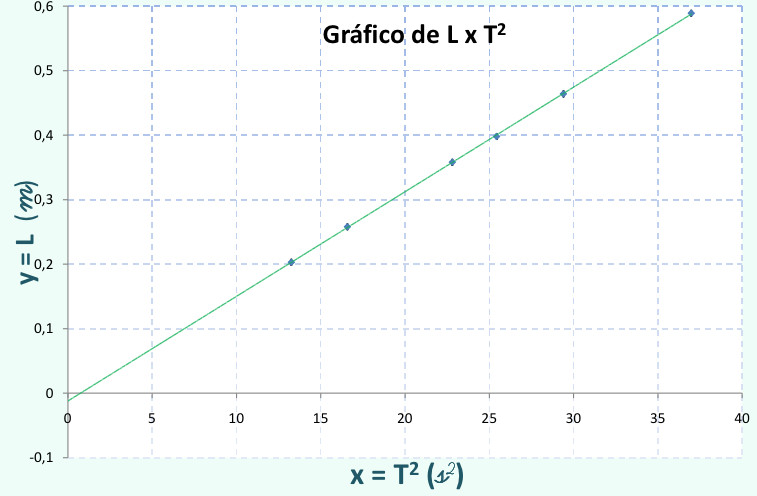
\includegraphics[scale=0.4]{2.jpg}
	\caption{Gráfico do comprimento do fio $L$ em função de $T^2$}
	\label{fig:grafico1}
\end{figure}

Portanto, sabendo que $r = (2,75\pm0,05) x 10^{-4}$ podemos aplicar na fórmula ~\ref{eq:CoeficienteLinear} e descobrir o valor de $G$, com erro propagado utilizando a seguinte fórmula:

\begin{align}
	 \sigma_{G}^2 = (8 \pi \frac{I_0}{r^4})^2 (\sigma_a)^2 + (8 \pi \frac{a}{r^4})^2(\sigma_{I_0})^2 + (-32 \pi \frac{aI_0}{r^5})^2 (\Delta_r)^2 
\end{align}

\subsection{Resultados}
Utilizando a fórmula obteve-se o seguinte resultado:
$$G \pm \sigma_G = (9,1 \pm 0,7) * 10^{10} \frac{N}{m^2} = 91\pm7 GPa$$
O valor esperado para o Aço ASTM, que foi o material usado é de aproximadamente 80 GPa. Ou seja, nosso valor e nossa faixa de erro estão um pouco maiores que o esperado. 

Algumas hipóteses que ajudam a justificar o erro, em ordem de maior para menor relevância: 
\begin{itemize}
	\item O estado do fio, que parecia ter sido dobrado e depois esticado, o que pode ter prejudicado ou modificado suas características de cisalhamento.
	\item Diferença na densidade dos cilindros, pois, para calcular o , supomos que os cilindros tivessem densidades iguais;
	\item Deslizamento e atrito entre o suporte e o fio, durante as rotações.
\end{itemize}

Para corrigir estes defeitos, o ideal seria obviamente usar cilindros de mesma densidade e um fio novo, sem defeitos e imperfeições significativas.

\section{Conclusão}

Ao final desse experimento, o módulo de cisalhamento $G$ obtido não está de acordo com o esperado, pelo que presumimos serem características do sistema montado, tais como a densidade desigual dos cilindros, imperfeições no fio e deslizamento entre o suporte e o fio. Porém o valor mínimo de nossa faixa de erro, 84 $GPa$ é razoavelmente próximo do esperado.

\end{document}